\section{Viscosity}

	[*Bhuvan: please add here the 'diagram-definition-viscosity']
	
	Viscosity is defined as,

	\[ \frac{F}{A} = \mu \left| \frac{dv}{dr} \right| \]

	$F$: shearing force on a surface of the layer, this force acts parallel to the surface plane.\\
	$A$: the area of the surface.\\
	$\mu$: coefficient of viscosity.\\
	$v$: velocity of the flow parallel to the plane.\\
	$r$: coordinate perpendicular to the plane.\\
	
	Diamension of viscosity,
	
	\[ [\mu] = \frac{[F]}{[A]} \frac{[r]}{[v]} \]
	
	\[ [\mu] = \frac{[ML/T^2]}{[L^2]} \frac{[L]}{[L/T]} \]
	
	\begin{equation} \label{eq:diamension-mu}
	[\mu] = \frac{M}{LT} = \frac{kg}{m.s}
	\end{equation}

\section{Volumetric flow rate through a thin tube}
	
	[*Bhuvan: please add here the 'diagram-flow-rate-cylinder']
	
	For a lamilar flow
	\[ force due to pressure gradient = viscous resistance \]
	
	\begin{equation}
	\boxed{Q = \frac{\pi}{8\mu}\frac{\Delta P}{l} R^4}
	\end{equation}
	$S$: cross-sectional area perpendicular to the flow.

	\begin{equation} \label{eq:flow-rate}
	\boxed{Q = \frac{\pi}{8\mu}\frac{\Delta P}{l} R^4}
	\end{equation}

\section{Flow rate in a tube containing meniscus}

	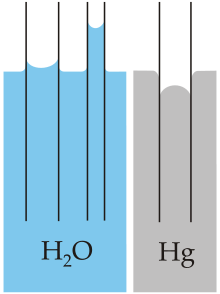
\includegraphics[height=5cm]{diagram/fig_capact-of-water} \label{fig_capact-of-water}

	Figure showing capillary action of water (polar) compared to mercury (non-polar), with respect to a polar surface such as glass (Si–OH). Let us apply this to our case, where the first node is filled with a fluid like water and the second node is filled with a fluid like air, and the our tube is similar to glass. Hence the meniscus will be oriented in a manner shown below.

	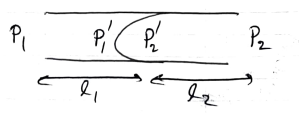
\includegraphics{diagram/fig_flowr-1-men}

	Let there be a higher pressure in $P_{1}$ than $P_{2}$, the fluid in node which has $P_{1}$ produces a meniscus whose tends move towards the second node. We can break it down into two separate tubes of lengths $l_{1}$ and $l_{2}$, containing fluid of viscosites ${\mu}_1$ and ${\mu}_2$. Then the flow rates for each of the tubes are given by:
	\begin{equation} \label{eq:flow-rate-first}
	Q_1 = \frac{\pi}{8{\mu}_1} \frac{P_1 - P^{'}_1}{l_1} R_1^4
	\end{equation}
	\begin{equation} \label{eq:flow-rate-second}
	Q_2 = \frac{\pi}{8{\mu}_2} \frac{P^{'}_2 - P_2}{l_2} R_2^4
	\end{equation}

	Multiplying equations \ref{eq:flow-rate-first} and \ref{eq:flow-rate-second} by ${\mu}_i l_i$
	\begin{equation} \label{eq:flow-rate-first-coeff}
	Q_1 {\mu}_1 l_1 = \frac{\pi}{8} (P_1 - P^{'}_1) R_1^4
	\end{equation}
	\begin{equation} \label{eq:flow-rate-second-coeff}
	Q_2 {\mu}_2 l_2 = \frac{\pi}{8} (P^{'}_2 - P_2) R_2^4
	\end{equation}

	Due to continuity, which means no vacuum or fluid can be created, $Q_1 = Q_2$. Since it is the same tube, $R_1 = R_2$. Adding equation \ref{eq:flow-rate-first-coeff} and \ref{eq:flow-rate-second-coeff}, we get:
	\begin{equation} \label{eq:flow-rate-intermediate}
	Q({\mu}_1 l_1 + {\mu}_2 l_2) = \frac{\pi}{8}R^4(P_1 - P_2 + P^{'}_2 - P^{'}_1)
	\end{equation}

	In figure \ref{fig_capact-of-water} the water rises because there is a pressure jump at the meniscus, the pressure is lower on the side of the water. Therefore in our case $P^{'}_2 - P^{'}_1$ will have a positive value. Equation \ref{eq:flow-rate-intermediate} becomes:
	\begin{equation}
	Q = \frac{\pi R^4}{8({\mu}_1 l_1 + {\mu}_2 l_2)}(\Delta P + \frac{2\sigma}{R})
	\end{equation}

	Let the node on which we are generating linear equations be $N_i$ and the node connected by a tube be $N_j$, if the concave side of the meniscus points towards $N_j$ from $N_i$, then let us say that the meniscus 'points away from $N_i$' or simply 'points away' and in the case of opposite orientation 'points towards'. Let the sign due to the orientation of meniscus be decided by a function called $sigmns(ort, n)$, where $ort$ is the orientation, and $n$ is the number of meniscus in the tube:
	\begin{equation}
	sigmns(ort, n) = 
	\begin{dcases}
	-1,&\text{ort points towards, n = 1}\\
	0,&\text{n = 0, 2}\\
	+1,&\text{ort points away, n = 1}
	\end{dcases}
	\end{equation}

	Finally we get:
	\begin{equation} 
	Q_{ij} = \frac{\pi R^3}{8({\mu}_1 l_1 + {\mu}_2 l_2)}(R\Delta P_{ij} + 2sigmns(ort, n)\sigma)
	\end{equation}

	It can be extended to the case when there are more than 1 meniscus, and using $s_{ij}$ for $sigmns_{ij}(ort, n)$:
	\begin{equation} \label{eq:flow-rate-main}
	\boxed{Q_{ij} = \frac{\pi R_{ij}^3}{8lM_{ij}}(R_{ij}\Delta P_{ij} + 2s_{ij}\sigma)}
	\end{equation}

	Here
	\[ M_{ij} = \sum\limits_{k}{\mu}_{ijk} \frac{l_{ijk}}{l} \]
	$Q_{ij}$ is the flow from $N_i$ to $N_j$ and $\Delta P_{ij} = P_i - P_j$. In case, when the flow is in the opposite direction $Q_{ij}$ will take the opposite sign.

	\begin{equation}
	Q_{ij} = -Q_{ji}
	\end{equation}


\section{The linear equations} \label{sec:linear-equ}

	Let us apply our method on a simple system consisting of only 5 nodes.

	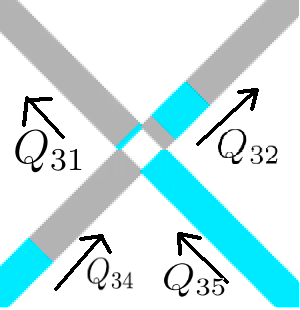
\includegraphics[height=6cm]{diagram/fig_simple-5-nodes}

	Since there are 4 tubes, we can write 4 equations according to \ref{eq:flow-rate-main}
	\[ Q_{31} = \frac{\pi R_{31}^3}{8lM_{11}}(R_{31}\Delta P_{31} + 2s_{31}\sigma) \]
	\[ Q_{32} = \frac{\pi R_{32}^3}{8lM_{12}}(R_{32}\Delta P_{32} + 2s_{32}\sigma) \]
	\[ Q_{34} = \frac{\pi R_{34}^3}{8lM_{14}}(R_{34}\Delta P_{34} + 2s_{34}\sigma) \]
	\[ Q_{35} = \frac{\pi R_{35}^3}{8lM_{15}}(R_{35}\Delta P_{35} + 2s_{35}\sigma) \]

	Since the sum of all $Q_{ij}$ is equal to zero. Then as we iterate for each tube connected to the node, in our case we have 4 tubes, it is sufficient to do the following three operations. Here let $K_{ij} = R^3_{ij}/{M}_{ij}$.

	\[ [P_i] + R_{ij}K_{ij} \]
	\[ [P_j] - R_{ij}K_{ij} \]
	\[ [const] - 2s_{ij}\sigma K_{ij} \]
	The matrix for Gaussian elimination will be

	\[ 
	\begin{pmatrix}
		1 & 0 & 0 & 0 & 0 & P_{up}\\
		0 & 1 & 0 & 0 & 0 & P_{up}\\
		-R_{31}K_{31} & -R_{32}K_{32} & (R_{3k}K_{3k} + ...) & -R_{34}K_{34} & -R_{35}K_{35} & -2\sigma(s_{3k}K_{3k} + ...)\\
		0 & 0 & 0 & 1 & 0 & P_{down}\\
		0 & 0 & 0 & 0 & 1 & P_{down}
	\end{pmatrix}
	\]
	 It can be proven that this matrix always has a solution. Once the solution is determined the flow rate can be calculated using equation \ref{eq:flow-rate-main}, and the velocity of flow in each tube is given by
	\begin{equation} \label{eq:velocity-in-tube}
	\boxed{v_{ij} = \frac{R_{ij}}{8lM_{ij}}(R_{ij}\Delta P_{ij} + 2s_{ij}\sigma)}
	\end{equation}
